\section{Поређење перформанси}
За мерење перформанси кориштени су примери судоку загонетки најтежег нивоа (\textit{evil}) димензија 9х9 и 16х16 и да би се додатно испровоцирао алгоритам за претрагу простора постојећих решења из тих примера обрисани су неки од бројева уз проверу да се њиховим брисањем није онемогућило решавање загонетке. Током тестирања мењан је број кориштених нити и процеса да би се уочио утицај паралелизације на брзину извршавања алгоритма. Модел процесора који је кориштен за тестирање је \textit{AMD Ryzen 7 7730U (base 2.0GHz, max 4.5GHz)}. Добијени су следећи резултати \ref{fig:seq_mp_results}\ref{fig:mpi_results}.

\begin{figure}[H]
    \centering
    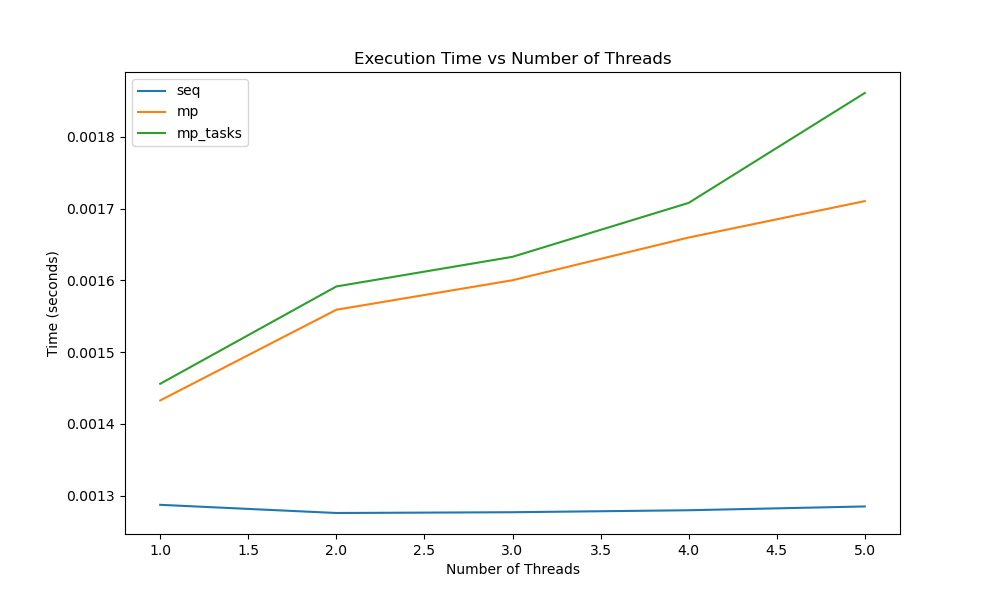
\includegraphics[width=1\textwidth]{images/graph_1.png}
    \caption{Резултати секвенцијалне и \textit{MP} имплементације}
    \label{fig:seq_mp_results}
\end{figure}

\begin{figure}[H]
    \centering
    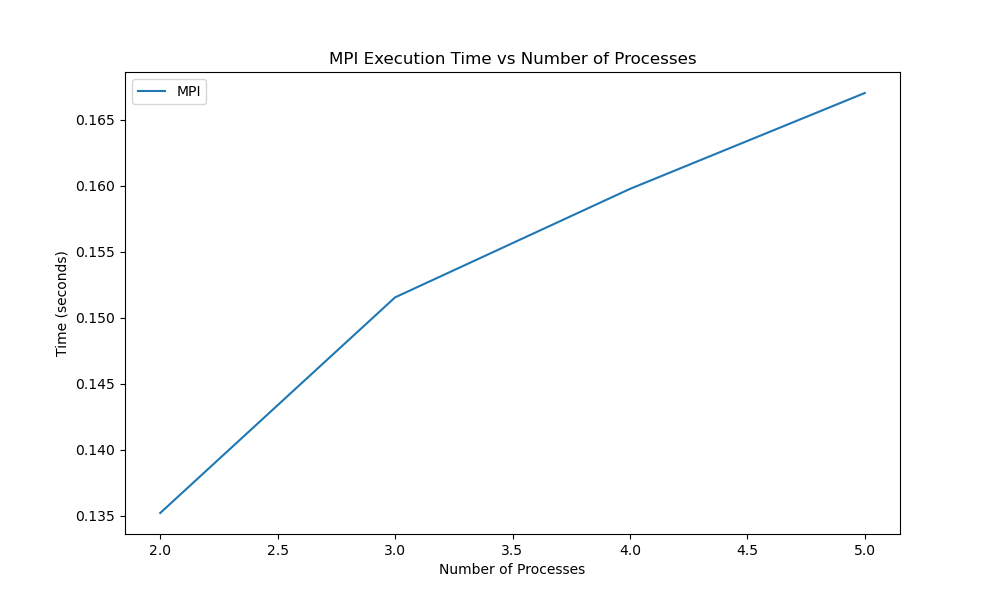
\includegraphics[width=1\textwidth]{images/graph_2.png}
    \caption{Резултати \textit{MPI} имплементације}
    \label{fig:mpi_results}
\end{figure}

На основу резултата да се уочити да је упркос разним покушајима паралелизације алгоритма за претрагу простора могућих решења, ипак секвенцијално решење најбрже и да се повећавањем броја нити и процеса само повећава \textit{overhead} потребан за координацију нити и процеса који додатно повећава време извршавања. Утицај на брзину секвенцијалног алгоритма највероватније има оптимизација алгоритма за пропагацију ограничења (проналажење оптималног кандидата и коришћење бинарног низа за складиштење могућих бројева), као и модернији модел процесора (мало мањи удео). Огромно одступање брзине \textit{MPI} имплементације оправдано је великим \textit{overhead}-ом који је потребан за координацију процеса, као и чинњеницом да се судоку матрица мора сваки пут трансформисати за потребе међусобне комуникације процеса, а њена величина није занемарљива.\\

Код \textit{OpenMP} имплементација може се приметити да је број итерација паралелизоване петље која се користи за претрагу простора могућих решења директно завистан од димензија судоку матрице, те је у примеру 9x9 матрице и највећи број итерација који се може јавити 9 што и не представља неки велики број итерација чак ни за секвенцијалну имплементацију. Могуће је да би \textit{OpenMP} имплементација имала боље перформансе у поређењу са секвенцијалном имплементацијом када би димензије матрице биле много веће, јер би у случају погрешне почетне претпоставке секвенцијална имплементација потрошила много времена док не исцрпи све случајеве и пређе на наредну претпоставку док би паралелна имплементација истовремено покушавала све претпоставке и прекинула извршавање по проналаску тачног решења  (детаљније објашњено у поглављу \ref{sec:parallel}).
